\section{Azure Stream Analytics}
Vor allem im heutigen Industrie 4.0 Umfeld sammeln sich schnell umfangreiche Datenmengen. Diese können oft nur über einen (stark) begrenzten Zeitraum zurückgehalten werden, da sie ansonsten ihre Aussagekraft verlieren. Ab diesem Punkt muss eine Datenverarbeitung erfolgen. Hier bietet Azure Stream Analytics eine Lösung. Dieser Dienst erlaubt Einblicke in Daten, um darin beispielsweise nach Mustern oder Anomalien zu suchen und entsprechend darauf zu reagieren \cite{Klein.2017}. Azure Stream Analytics unterstützt dabei eine SQL-Ähnliche Abfragesprache Stream Analytics Query Language (SAQL), über welche man die dynamischen Datenströme analysiert. Diese ist das Herzstück des Dienstes. Obwohl SAQL von der allgegenwärtigen SQL-Abfragesprache abgeleitet wurde, enthält es einzigartige Funktionen, die für die Stream-Verarbeitung notwendig sind \cite{Prosise.}. Eine dieser Funktionen ist die Möglichkeit, Ergebnisse mithilfe von Zeitfenstern zu erhalten (siehe Fensterfunktionen). Ein typisches Echtzeitverarbeitungssystem, welches auf Stream Analytics und weiteren Azure-Diensten aufbaut, ist in Abbildung \ref{uebersicht} aufgeführt.
\begin{figure*}[ht]
	\centering
	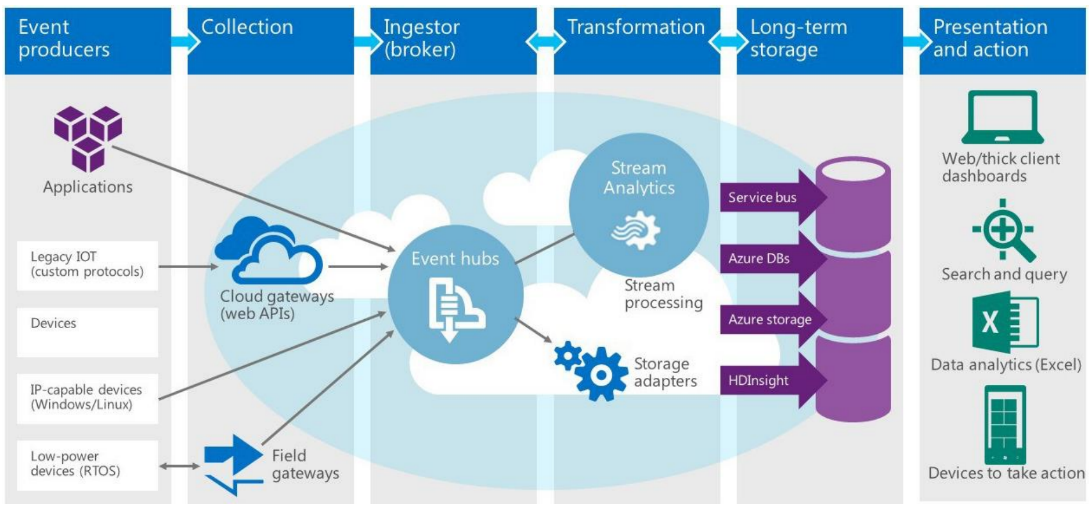
\includegraphics[width=0.8\textwidth,]{images/StreamAnalytics}
	\caption{Typisches Echtzeitverarbeitungssystem \cite{Prosise.}}
	\label{uebersicht}
\end{figure*}
\\ \\Die linke Spalte zeigt Sensoren, Geräte und andere Datenquellen einer IoT-Lösung. Diese senden permanent Daten über das Cloud Gateway an die Azure Hubs. Der Gateway-Dienst ist hierbei ein virtuelles Gerät und ermöglicht eine konsistente Verbindung. Die Hubs sind in der Lage Millionen von Ereignissen pro Sekunde zu verarbeiten. Von dort aus werden sie an die weiteren Anwendungen übergeben. Stream Analytics transformiert eingehenden Daten. Die Ausgaben lassen sich daraufhin auf eine Vielzahl von Endpunkten richten. Azure bietet hier einige Dienste, welche daran angeknüpft werden können \cite{Prosise.}. \\
Sowohl Ein- als auch Ausgaben, die ein Stream Analytics-Job benötigt, werden im Azure-Portal konfiguriert. Ein einzelner Stream Analytics-Job kann mehrere Eingaben enthalten. Durch Aggregation der Datenströme lassen sich kombinierte Abfragen durchführen. Dies kann mit einem JOIN in SQL verglichen werden. Dadurch, dass ein einzelner Stream Analytics-Job mit mehreren Ein- und Ausgängen konfiguriert werden kann, ermöglicht umfangreiche Topologien \cite{Prosise.}. Zur Verfügung stehen hier Services wie:
\begin{itemize}
	\item Azure-Event-Hub
	\item Azure-IoT-Hub
	\item Azure-Blobspeicher 
	\item Azure-Tabellenspeicher 
	\item Azure-Ereignis-Hub 
	\item Azure-Servicebus-Thema 
	\item Azure Service Bus-Warteschlange 
	\item Azure DocumentDB 
	\item Microsoft Power BI 
	\item Azure Data Lake Store 
\end{itemize} 